\documentclass{article}
\usepackage{graphicx}
\usepackage[margin=2.5cm]{geometry}
\usepackage[labelfont=bf]{caption}
\usepackage{color}
\usepackage{xcite}
\usepackage{amsmath}
%\usepackage{natbib}
\usepackage{subcaption}
\usepackage{multirow}

\renewcommand{\textfraction}{1.0}
\renewcommand{\floatpagefraction}{.9}
\newcommand\revised[1]{\textcolor{red}{#1}}
\usepackage[nomarkers,nofiglist,notablist]{endfloat}

%\def \@largefloatcheck{\ht\@currbox 0.5\textheight}
%\renewcommand{\topfraction}{0.9}    % max fraction of floats at top
%\renewcommand{\bottomfraction}{0.8} % max fraction of floats at bottom
%\renewcommand{\textfraction}{0.01}  % allow minimal text w. figs

\makeatletter 
\renewcommand{\thefigure}{S\@arabic\c@figure} 
\renewcommand{\thetable}{S\@arabic\c@table} 

\newcommand{\figdeconv}{4}

\externalcitedocument{betternorm}

\usepackage{url}
\urlstyle{same}

\begin{document}

\begin{titlepage}
\vspace*{3cm}
\begin{center}

{\LARGE
Much ado about nothing: how to normalize single-cell RNA sequencing data with many zero counts
\par}

\vspace{0.75cm}

{\Large 
    \textsc{Supplementary Materials}
\par
}
\vspace{0.75cm}

\large
by

\vspace{0.75cm}
Aaron T. L. Lun$^{1}$, Karsten Bach$^{2}$ and John C. Marioni$^{1,2}$

\vspace{1cm}
\begin{minipage}{0.9\textwidth}
\begin{flushleft} 
$^1$Cancer Research UK Cambridge Institute, University of Cambridge, Li Ka Shing Centre, Robinson Way, Cambridge CB2 0RE, United Kingdom \\[6pt]
$^2$EMBL European Bioinformatics Institute, Wellcome Genome Campus, Hinxton, Cambridge CB10 1SD, United Kingdom \\[6pt]
\end{flushleft}
\end{minipage}

\vspace{1.5cm}
{\large \today{}}

\vspace*{\fill}
\end{center}
\end{titlepage}

\begin{figure}[btp]
    \begin{center}
        \begin{minipage}{0.4\textwidth}
            \includegraphics[width=\textwidth,trim=0mm 5mm 2mm 5mm,clip]{../realdata/Klein_Means.pdf}
            \subcaption{}\label{subfig:kleinmean}
        \end{minipage}
        \begin{minipage}{0.4\textwidth}
            \includegraphics[width=\textwidth,trim=0mm 5mm 2mm 5mm,clip]{../realdata/Klein_Dispersions.pdf}
            \subcaption{}\label{subfig:kleindisp}
        \end{minipage}
    \end{center}
    \caption{
        Parameter estimates for the Klein \textit{et al.} data set \cite{klein2015droplet}.
        (\subref{subfig:kleinmean}) Histogram of average counts for all genes. 
        The red curve represents the probability density of a Gamma$(2, 2)$ distribution.
        (\subref{subfig:kleindisp}) Smoothed scatter plot of NB dispersion estimates from edgeR, plotted against the average count.
        Axes are log-transformed for visibility.
        The dashed line represents the fitted trend from edgeR, while the unbroken line is drawn at 0.1.
    }
\end{figure}

\begin{figure}[btp]
    \begin{center}
        \begin{minipage}{0.33\textwidth}
            \includegraphics[width=\textwidth,trim=0mm 14mm 2mm 20mm,clip]{../simulations/results/sizeP_1.pdf}
            \includegraphics[width=\textwidth,trim=0mm 14mm 2mm 20mm,clip]{../simulations/results/sizeP_4.pdf}
            \subcaption{}\label{subfig:size_prior}
        \end{minipage}
        \begin{minipage}{0.33\textwidth}
            \includegraphics[width=\textwidth,trim=0mm 14mm 2mm 20mm,clip]{../simulations/results/sizeP2_1.pdf}
            \includegraphics[width=\textwidth,trim=0mm 14mm 2mm 20mm,clip]{../simulations/results/sizeP2_4.pdf}
            \subcaption{}\label{subfig:size_libprior}
        \end{minipage}
    \end{center}
    \caption{
        Performance of DESeq normalization after addition of a pseudo-count.
        A pseudo-count of unity was added to (\subref{subfig:size_prior}) all counts directly, or (\subref{subfig:size_libprior}) after scaling the pseudo-count by the relative library size, i.e., the pseudo-count added to each cell was equal to the ratio of its library size to the mean library size.
        Simulations were performed with no DE (first row) and varying magnitudes of DE (second row).
        Axes are shown on a log-scale.
        For comparison, each set of size factors was scaled such that the grand mean across cells was the same as that for the true values.
        The red line represents equality between the rescaled estimates and true factors.
        Cells in the first, second and third subpopulations are shown in black, blue and orange, respectively.
    }
\end{figure}

\revised{\section{Justifying the choice of pooling strategy}
The performance of a ring arrangement and sliding window can be compared to selection of random pools of cells.
Count data was simulated as described in the main text, with some modifications -- specifically, true values of $\theta_j$ for all cells were sampled from a Uniform(0.1, 1) distribution instead, to provide a larger range of size factors; counts were only generated for a single subpopulation of 200 cells; and no DE genes were introduced.
To estimate the size factors, deconvolution was performed using pools of 20 cells, assembled either with the ring arrangement in Figure~\ref{fig:library_ring} or after randomly permuting the order of cells in the ring.
(For demonstration purposes, only one pool size was used to construct the linear system.
This ensures that the estimation errors are large enough to reliably observe any changes in precision.)
Precision was quantified as the median absolute deviation (MAD) of the log-fold differences between the estimated and true $\theta_j$.
A completely precise method should have a MAD of zero, as the estimated and true $\theta_j$ would be proportionally identical for all $j$.
In this simulation, using the ring arrangement yields a MAD of 0.051 while using random pools yields a MAD of 0.079 (standard errors of 0.002 and 0.003, respectively, across 10 simulation iterations).
This suggests that the ring arrangement provides a modest improvement in estimation precision.
}


\begin{figure}[btp]
    \begin{center}
        \includegraphics[width=0.5\textwidth]{pics/library_ring.pdf}
    \end{center}
    \caption{
        Ring arrangement of cells ordered by library size.
        Each circle represents a cell where the size of the circle corresponds to the library size of that cell.
        Even- and odd-ranking cells lie on opposite sides, with the largest and smallest libraries at the top and bottom, respectively.
        Cells lying in a window of length 4 are highlighted in red.
        Different instances of the window are obtained by sliding the window across the ring.
    }
    \label{fig:library_ring}
\end{figure}


\section{Resolving linear dependencies in the constructed system}
Consider the application of the deconvolution method on a data set with four cells using a sliding window of size 2.
Assuming cells $j=1$ to $4$ were placed consecutively on the ring, this would yield the linear system
\[
\begin{bmatrix}
1 & 1 & 0 & 0 \\
0 & 1 & 1 & 0 \\
0 & 0 & 1 & 1 \\
1 & 0 & 0 & 1 
\end{bmatrix}
\begin{bmatrix}
\theta_1 \\
\theta_2 \\
\theta_3 \\
\theta_4 
\end{bmatrix}
=
\begin{bmatrix}
\theta_A \\
\theta_B \\
\theta_C \\
\theta_D 
\end{bmatrix}
\]
for pool-based size factor estimates $\theta_A$ to $\theta_D$. 
Assume that the pool-based factors are estimated accurately and precisely, such that the minimum value of the residual sum of squares for this system can be obtained near the set of true values for the cell-based factors.
This system has no unique solution - for the true factors $(\theta_1, \theta_2, \theta_3, \theta_4)^T$, 
    an equally good fit can be obtained with $(\theta_1+x, \theta_2-x, \theta_3+x, \theta_4 - x)^T$ for any real $x$.

The addition of equations relating each $\theta_j$ with its direct estimate $\theta'_j$ ensures identifiability, 
    as a value of $x$ will be chosen that minimizes the residual sum of squares of the $(\theta_1+x, \theta_2-x, \theta_3+x, \theta_4 - x)^T$ from the direct estimates.
In this example, the residual sum of squares for the possible solutions can be written as
\[
\sum_{j \in J_1} (\theta_j +x - \theta'_j)^2+ \sum_{j \in J_2} (\theta_j -x - \theta'_j)^2 
= 4 x^2 + 2x\left[ \sum_{j \in J_1} (\theta_j - \theta'_j) - \sum_{j \in J_2} (\theta_j - \theta'_j)\right] + \sum_{j \in \{J_1, J_2\}} (\theta_j - \theta'_j)^2
\]
where $J_1 = \{1, 3\}$ and $J_2=\{2, 4\}$.
For these 4 cells, the above expression is minimized in terms of $x$ at
\[
x = - \frac{1}{4}\left[ \sum_{j \in J_1} (\theta_j - \theta'_j) - \sum_{j \in J_2} (\theta_j - \theta'_j)\right] \;.
\]
The direct estimate of each size factor is unbiased as stochastic zeroes are not removed, i.e., $E(\theta_j - \theta'_j)=0$.

As the number of cells in the system increases, the sizes of $J_1$ and $J_2$ will increase. 
For example, deconvolution is typically applied in data sets involving at least 200 cells and a sliding window of size 20, such that both $J_1$ and $J_2$ will consist of at least 10 cells.
With more cells, the sum of the errors $\theta_j - \theta'_j$ will approach the sum of their expected values, i.e., zero.
This means that the minimum residual sum of squares will be obtained at $x=0$, i.e., solving the linear system will yield the true values of the size factors.
Thus, the additional equations will not affect accurate estimation of the size factors in the deconvolution method.

\section{Implementation details of the clustering approach}
Let $\rho_{xy}$ denote Spearman's rank correlation coefficient between the counts of cells $x$ and $y$.
We define the distance between these cells as $1-\rho_{xy}$.
In this manner, a distance matrix is constructed between all pairs of cells.
Hierarchical clustering is performed on this matrix using the hclust function with Ward's clustering criterion.
Clusters of cells are defined using a dynamic tree cut from the dynamicTreeCut package v1.62 ({https://cran.r-project.org/web/packages/dynamicTreeCut/index.html}).
This ensures that each cluster contains a minimum number of cells (200 by default) required for stable deconvolution.
Correlation-based clustering is appealing as it is insensitive to global scaling of the expression values in each cell.
Prior normalization is not required, which avoids a circular dependence between normalization and clustering.
Alternatively, one can use known aspects of the data set as clusters, e.g., groupings, batches.
Empirical clustering may not be required if such information is available, which reduces computational work and reduces the potential for errors.

% While PCA does mean-centering of each gene, this is probably unwise for correlation-based clustering. 
% Two cells that are similar to the mean expression profile will have uncorrelated residuals and would appear to be unrelated. 
% The correct correlation should be near unity as their expression values would match up perfectly. 
% Use of uncentered counts is also easier to interpret and ensures insensitivity to normalization.

By default, the baseline pseudo-cell is chosen from the cluster where the mean library size per cell is equal to the median of the mean library size across all clusters
    (or, for an even number of clusters, the cluster with the smallest mean library size above the median).
This uses the mean library size as a rough proxy for cell similarity.
The baseline cluster is likely to be least dissimilar to every other cluster, which reduces the amount of DE during pairwise normalization between pseudo-cells.
More intelligent choices of the baseline can be used if the similarities between clusters are known, e.g., from visualization after dimensionality reduction.

In general, cluster-specific normalization requires some caution.
Done incorrectly, this may introduce artificial differences between cells in different clusters, 
    such that the statistical rigour of downstream analyses (e.g., to detect DE between clusters) would be compromised.
However, such problems are avoided here by using a two-step normalization strategy.
The first normalization step removes any systematic differences between cells \textit{within} each cluster, 
    while the second normalization between pseudo-cells removes any differences \textit{between} clusters.
The end result is that differences between all cells in all clusters are removed.
This is equivalent to the outcome of a hypothetical one-step method that does not use cluster information (and is robust to DE and stochastic zeroes, unlike existing methods).
Moreover, normalization accuracy in Figure~\figdeconv{} is unaffected by the use of clustering prior to deconvolution, which suggests that this approach is valid.

Semi-systematic zeroes may be removed prior to deconvolution in each cluster.
In particular, genes are removed if they only have zero counts across all cells in the cluster.
Such genes provide no information for normalizing between cells in the same cluster, and their removal will not affect the cluster-specific size factor estimates.
However, these genes are retained during rescaling of the size factors between clusters.
This is because they will have non-zero counts in at least one cluster (assuming that systematic zeroes across the entire data set have already been removed).
Removal of such genes will distort the median ratio between pseudo-cells and lead to biased size factor estimates, as described previously for the existing methods.

\revised{\section{Assessing normalization in high-coverage simulations}
The simulations in the main text represent low-coverage experiments similar to the Zeisel \textit{et al.} and Klein \textit{et al.} data sets.
However, many scRNA-seq experiments involve higher sequencing coverage, e.g., over $2\times 10^5$ reads per cell \cite{kolod2015single}, compared to approximately $2\times10^4$ in low-coverage experiments.
To test the performance of deconvotluion and the existing normalization methods in high-coverage scenarios, we repeat the simulations with some modifications.
In particular, we redefine the sampling distribution of $\lambda_{i0}$ such that 
\[
    \log_2(\lambda_{i0}) \sim \mbox{Uniform}(3, 6) \;.
\]
This provides a wider spread of abundances than in the original simulation, as the dynamic range of sequencing counts increases with coverage.
The NB dispersion is also re-defined for each gene as 
\[
    \varphi_i = 2 + \frac{100}{\lambda_{i0}}
\]
to represent a decreasing mean-dispersion trend.
Large values for $\varphi_i$ are consistent with the high levels of technical noise and biological heterogeneity in scRNA-seq data, and ensure that a large number of stochastic zeroes are generated.
Counts are then sampled for a NB distribution with a mean of $\theta_{j}\lambda_{is}$ and dispersion $\varphi_i$.}

\revised{Simulated data were generated using the same experimental designs as described in the main text.
For the existing methods, similar performance was observed here compared to the original simulations.
DESeq and TMM normalization are consistently biased (Figures~\ref{subfig:sizehighcov} and \ref{subfig:tmmhighcov}), suggesting that zero counts are still problematic in high coverage data sets.
Library size normalization continues to fail in the presence of DE genes (Figure~\ref{subfig:libhighcov}).
In contrast, deconvolution performs well in all simulation scenarios (Figure~\ref{fig:highcovdeconv}).
Greater divergence from the true size factors is observed in Figure~\ref{subfig:sumclust_3}, but deconvolution is still more accurate than the existing methods in the equivalent scenario (Figure~\ref{fig:highcovexisting}, third row).
These results suggest that the increase in normalization accuracy from deconvolution is still present in higher-coverage experiments.
}

\newcommand{\results}{../simulations/results_mid}

\begin{figure}[btp]
\begin{minipage}{0.33\textwidth}
\includegraphics[width=\textwidth,trim=0mm 14mm 2mm  5mm,clip]{\results/size_1.pdf}
\includegraphics[width=\textwidth,trim=0mm 14mm 2mm 20mm,clip]{\results/size_2.pdf}
\includegraphics[width=\textwidth,trim=0mm 14mm 2mm 20mm,clip]{\results/size_3.pdf}
\includegraphics[width=\textwidth,trim=0mm  5mm 2mm 20mm,clip]{\results/size_4.pdf}
\subcaption{}\label{subfig:sizehighcov}
\end{minipage}
\begin{minipage}{0.33\textwidth}
\includegraphics[width=\textwidth,trim=0mm 14mm 2mm  5mm,clip]{\results/TMM_1.pdf}
\includegraphics[width=\textwidth,trim=0mm 14mm 2mm 20mm,clip]{\results/TMM_2.pdf}
\includegraphics[width=\textwidth,trim=0mm 14mm 2mm 20mm,clip]{\results/TMM_3.pdf}
\includegraphics[width=\textwidth,trim=0mm  5mm 2mm 20mm,clip]{\results/TMM_4.pdf}
\subcaption{}\label{subfig:tmmhighcov}
\end{minipage}
\begin{minipage}{0.33\textwidth}
\includegraphics[width=\textwidth,trim=0mm 14mm 2mm  5mm,clip]{\results/lib_1.pdf}
\includegraphics[width=\textwidth,trim=0mm 14mm 2mm 20mm,clip]{\results/lib_2.pdf}
\includegraphics[width=\textwidth,trim=0mm 14mm 2mm 20mm,clip]{\results/lib_3.pdf}
\includegraphics[width=\textwidth,trim=0mm  5mm 2mm 20mm,clip]{\results/lib_4.pdf}
\subcaption{}\label{subfig:libhighcov}
\end{minipage}
\caption{
    Performance of existing normalization methods in high-coverage simulations with DE genes and stochastic zeroes.
    The size factor estimates for all cells are plotted against the true values for (\subref{subfig:sizehighcov}) DESeq, (\subref{subfig:tmmhighcov}) TMM and (\subref{subfig:libhighcov}) library size normalization.
    Simulations were performed with no DE (first row), moderate DE (second row), strong DE (third row) and varying magnitudes of DE (fourth row).
    Axes are shown on a log-scale.
    For comparison, each set of size factors was scaled such that the grand mean across cells was the same as that for the true values.
    The red line represents equality between the rescaled estimates and true factors.
    Cells in the first, second and third subpopulations are shown in black, blue and orange, respectively.
}
\label{fig:highcovexisting}
\end{figure}

\begin{figure}[btp]
\begin{center}
\begin{minipage}{0.33\textwidth}
\includegraphics[width=\textwidth,trim=0mm 5mm 0mm 17mm,clip]{\results/sumClust_1.pdf}
\subcaption{}\label{subfig:sumclust_1}
\end{minipage}
\begin{minipage}{0.33\textwidth}
\includegraphics[width=\textwidth,trim=0mm 5mm 0mm 17mm,clip]{\results/sumClust_2.pdf}
\subcaption{}\label{subfig:sumclust_2}
\end{minipage}  \\ 
\begin{minipage}{0.33\textwidth}
\includegraphics[width=\textwidth,trim=0mm 5mm 0mm 17mm,clip]{\results/sumClust_3.pdf}
\subcaption{}\label{subfig:sumclust_3}
\end{minipage}
\begin{minipage}{0.33\textwidth}
\includegraphics[width=\textwidth,trim=0mm 5mm 0mm 17mm,clip]{\results/sumClust_4.pdf}
\subcaption{}\label{subfig:sumclust_4}
\end{minipage}
\end{center}
\caption{Size factor estimates from the deconvolution method in the high-coverage simulations,
    shown against the true values for scenarios with (\subref{subfig:sumclust_1}) no DE, (\subref{subfig:sumclust_2}) moderate DE, (\subref{subfig:sumclust_3}) strong DE and (\subref{subfig:sumclust_4}) varying magnitude of DE.
    Cells in the first, second and third subpopulations are shown in black, blue and orange, respectively.
    Axes are shown on a log-scale, and the red line represents equality with the true factors.
}
\label{fig:highcovdeconv}
\end{figure}

\revised{\section{Computational complexity of the deconvolution method}
The computational time and memory required by deconvolution depend on the number of cells.
An equation is constructed for each cell, so the size of the linear system (in terms of the number of equations and coefficients) will increase quadratically with the number of cells.
Furthermore, common implementations of the QR decomposition have $O(n^3)$ time complexity for $n$ cells.
This is roughly consistent with our empirical timings (Figure~\ref{fig:timings}).
In practice, the cubic time complexity is mitigated by the use of clustering to break up the linear system.
As deconvolution is performed within each cluster, it is cubic only with respect to the size of each cluster, and is linear with respect to the number of clusters.
The overall time complexity lies between the linear and cubic extremes, depending on the number of clusters and size of each cluster 
    -- a few large clusters will result in cubic complexity, while many small clusters will result in linear complexity.}

\begin{figure}[btp]
    \begin{center}
        \includegraphics[width=0.5\textwidth]{../simulations/timings.pdf}
    \end{center}
    \caption{
        Computational time used by deconvolution on a simulated data set with varying numbers of cells.
        Counts were sampled from a Poisson distribution with a mean of 10, for 10000 genes across 200-800 cells.
        Deconvolution was applied with and without separation into clusters of 200 cells.
        This was repeated for 10 simulation iterations, where each line in the plot represents the timings for one iteration.
    }
    \label{fig:timings}
\end{figure}

\revised{Memory usage of the deconvolution method is harder to assess due to the unpredictability of garbage collection in R.
We expect that usage will increase quadratically with the number of cells, due to the size of the linear system.
Again, this can be mitigated by clustering for large data sets.
Further savings may be possible by using sparse matrices given that most of the entries in the system are likely to be zero.}

\revised{We note that most clustering algorithms have quadratic time complexity with respect to the number of cells, e.g., when building the distance matrix.
However, we expect that clustering would be performed anyway as a routine part of the scRNA-seq data analysis.
Thus, no additional time is added by normalization.}
   
%\section{Deconvolution is inconsistent with spike-in normalization}
%The brain data set also contains counts for ERCC spike-in genes that are commonly used for normalizing scRNA-seq data.
%Briefly, a constant quantity of spike-in RNA is added to each cell and processed with the cellular RNA \cite{stegle2015computational}.
%Upon sequencing and quantification, differences in the coverage of spike-in genes between cells are interpreted as cell-specific biases and removed.
%At its simplest, spike-in normalization uses the total count across the spike-in genes as the size factor for each cell.
%This is similar to library size normalization with the counts for the cellular genes, but is more robust as no DE is expected across cells for a constant spike-in set.
%Problems with stochastic zeroes are avoided, and the assumption of a non-DE majority is not required.
%However, spike-in normalization does assume that the same quantity of spike-in RNA can be added to each cell \cite{robinson2010scaling,marinov2014singlecell}.
%It also assumes that the spike-ins behave similarly to the cellular transcripts \cite{grun2015design}.
%Violations of these assumptions may compromise performance, as observed in some bulk RNA-seq data sets \cite{risso2014normalization}.
%
%Examination of the data indicates that no correlation -- qualitative or quantitative -- 
%    exists between the sets of size factors from spike-in and the other normalization methods (Figure~\ref{fig:real_spike}).
%This is attributable to the differences in the underlying assumptions of each method.
%If most genes are DE, deconvolution and the existing methods will be incorrect and spike-in normalization will be more accurate.
%Conversely, spike-in normalization will be incorrect if spike-ins are not added precisely or if spike-in and cellular transcripts behave differently during library preparation.
%These results suggest that the validity of each assumption requires some consideration before normalization.
%For example, the similarity of the input cell types can be used to gauge the appropriateness of the non-DE assumption. 
%Here, over half of the cells are classified as neuronal \cite{zeisel2015brain}, so a non-DE majority of genes is not entirely unreasonable.
%Obviously, the truth of each assumption is largely unknown, so it is difficult to definitively determine the correct method for any given data set.
%
%\begin{figure}[btp]
%\begin{center}
%    \begin{minipage}{0.33\textwidth}
%        \includegraphics[width=\textwidth,trim=0mm 5mm 0mm 15mm,clip]{../realdata/Zeisel_ERCCvSF.pdf}
%        \subcaption{}\label{subfig:spike_sf}
%    \end{minipage}
%    \begin{minipage}{0.33\textwidth}
%        \includegraphics[width=\textwidth,trim=0mm 5mm 0mm 15mm,clip]{../realdata/Zeisel_ERCCvTMM.pdf}
%        \subcaption{}\label{subfig:spike_tmm}
%    \end{minipage} \\ 
%    \begin{minipage}{0.33\textwidth}
%        \includegraphics[width=\textwidth,trim=0mm 5mm 0mm 15mm,clip]{../realdata/Zeisel_ERCCvLib.pdf}
%        \subcaption{}\label{subfig:spike_lib}
%    \end{minipage} 
%    \begin{minipage}{0.33\textwidth}
%        \includegraphics[width=\textwidth,trim=0mm 5mm 0mm 15mm,clip]{../realdata/Zeisel_ERCCvDeconv.pdf}
%        \subcaption{}\label{subfig:spike_sum}
%    \end{minipage}
%\end{center}
%    \caption{
%        Comparisons between the estimated size factors from spike-in normalization to those from (\subref{subfig:spike_sf}) DESeq, (\subref{subfig:spike_tmm}) TMM,
%            (\subref{subfig:spike_lib}) library size normalization or (\subref{subfig:spike_sum}) the deconvolution method for all cells in the brain data set.                  
%        All sets of size factors were scaled to have a median of unity.
%        Axes are shown on a log-scale.
%    }
%    \label{fig:real_spike}  
%\end{figure}
%
%Of greater biological relevance is the fact that spike-in normalization preserves differences in cell size and total RNA content.
%In contrast, deconvolution and the existing methods will remove such differences.
%This is because they affect all genes within each cell and are subsequently treated as part of the cell-specific bias.
%Whether or not this is appropriate depends on whether cell size differences are of interest to the researcher.
%In some scenarios, this may be the case such that spike-ins should be used, e.g., when studying cycling cells with differences in total RNA.
%For other applications, cell size may be a confounding variable that needs to be removed.
%For these data sets, normalization should be performed with the deconvolution method.
%
%Ideally, the decision to use spike-ins or not should be driven by biology, i.e., whether cell size is relevant to the study.
%In practice, however, issues such as cost and convenience dictate whether spike-ins are added in the experiment.
%This is especially true for droplet-based protocols \cite{macosko2015highly,klein2015droplet} for which the consistent incorporation of spike-ins is not straightforward.
%If spike-ins are not available, normalization of cell-specific biases must be performed with methods that assume a non-DE majority, e.g., TMM, deconvolution.

\begin{table}[p]
    \caption{
        Proportion of the top set of DE genes that were shared between deconvolution and each existing normalization method.
        Top genes were identified as those with the lowest $p$-values from edgeR in the analysis with each normalization method.
        Top sets of size ranging from 100 to 2000 were tested for both the brain and inDrop data sets.
        Smaller sets were not tested due to avoid ambiguous ranks from $p$-values of zero.
    }
    \begin{center}
        \begin{tabular}{l r r r r}
            \hline
            \multirow{2}{*}{\textit{Data set}} & \multirow{2}{*}{\textit{Top}} & \multicolumn{3}{c}{\textit{Method}} \\
                \cline{3-5}
                & & DESeq & TMM & Library size \\
            \hline
            \multirow{3}{*}{Brain}            
            & 100  & 0.44 & 0.60 & 0.71 \\ 
            & 500  & 0.60 & 0.70 & 0.75 \\
            & 2000 & 0.70 & 0.75 & 0.80 \\
            \hline
            \multirow{3}{*}{inDrop}            
            & 100  & 0.88 & 0.94 & 0.98 \\ 
            & 500  & 0.84 & 0.92 & 0.97 \\
            & 2000 & 0.83 & 0.93 & 0.95 \\
            \hline
        \end{tabular}
    \end{center}
\end{table}

\begin{table}[p]
    \caption{ 
        Proportion of the top set of highly variable genes that were shared between deconvolution and each existing normalization method.
        Top genes were identified as those with the largest distance-to-median values. 
        For both data sets, top sets of size ranging from 100 to 2000 were compared between methods.
    }
    \begin{center}
        \begin{tabular}{l r r r r}
            \hline
            \multirow{2}{*}{\textit{Data set}} & \multirow{2}{*}{\textit{Top}} & \multicolumn{3}{c}{\textit{Method}} \\
                \cline{3-5}
                & & DESeq & TMM & Library size \\
            \hline
            \multirow{3}{*}{Brain}            
            & 100  & 0.78 & 0.81 & 0.90 \\ 
            & 500  & 0.78 & 0.80 & 0.88 \\
            & 2000 & 0.67 & 0.73 & 0.84 \\
            \hline
            \multirow{3}{*}{inDrop}            
            & 100  & 0.74 & 0.76 & 0.90 \\ 
            & 500  & 0.57 & 0.59 & 0.85 \\
            & 2000 & 0.59 & 0.61 & 0.85 \\
            \hline
        \end{tabular}
    \end{center}
\end{table}

\revised{\section{Comparing normalization accuracy on real data}
Consider two sets of size factor estimates, $\hat\theta_j$ and $\hat\theta'_j$ for each cell $j$.
We assume that $\log(\hat\theta_j)$ is an unbiased estimator of the true log-value, i.e., $E[\log(\hat\theta_j)] = \log(\theta_j)$ for the true size factor $\theta_j$ in cell $j$.
In contrast, we define $\hat\theta'_j$ to exhibit estimation bias such that a power relationship exists between the estimates and true values.
This is not unreasonable given the simulation results (Figure~\ref{fig:highcovexisting}), and can be written as
\[
    E[\log(\hat\theta_j)] = b \log(\theta'_j) + c
\]
for gradient $b$ and some constant $c$. 
Any bias will manifest as a non-unity gradient indicating divergence between the true and estimated values.
For simplicity, we scale the values of $\theta'_j$ such that $c=0$. 
(This does not affect the generality of the framework, as the absolute scale of the size factors is irrelevant to their interpretation.)
We define the true mean for gene $i$ in cell $j$ as $\mu_{ij} = \theta_j\lambda_{i0}$, where $\lambda_{i0}$ represents the expected number of transcripts.
We assume that no DE is present, so a constant $\lambda_{i0}$ can be used for all cells.}

\revised{Now, consider fitting a log-link GLM to the counts using $\log(\hat\theta_j)$ as an offset and $\log(\hat\theta'_j)$ as the only covariate in a model with an intercept term.
The fitted value would be $\log(\hat\theta_j) + \hat\beta_{i0} + \log(\hat\theta'_j)\hat\beta_{i1}$, where $\hat\beta_{i0}$ and $\hat\beta_{i1}$ are the estimates of the coefficients for the intercept and covariate terms, respectively.
If we were to equate the expectation of the fitted value to the log-transformed true mean, we would obtain
\begin{align*}
    \log(\mu_{ij}) &= E[\log(\hat\theta_j) + \hat\beta_{i0} + \log(\hat\theta'_j)\hat\beta_{i1}] \\
    \log(\theta_j) + \log(\lambda_{i0}) &=  \log(\theta_j) + \hat\beta_{i0} + b \log(\theta_j) \hat\beta_{i1} \\
    \log(\theta_j) &=  \log(\theta_j) + b \log(\theta_j)\hat\beta_{i1} \qquad\mbox{as $\hat\beta_{i0}$ absorbs all terms without $j$}\\
    \hat\beta_{i1} &= 0 
\end{align*}
assuming that $b' \log(\theta_j)$ are non-zero. 
Dropping the covariate term and performing a likelihood ratio test (LRT) should yield few DE genes.
In contrast, using $\log(\hat\theta'_j)$ as the offset and $\log(\hat\theta_j)$ as the covariate yields 
\begin{align*}
    \log(\mu_{ij}) &= E[\log(\hat\theta'_j) + \hat\beta'_{i0} + \log(\hat\theta_j)\hat\beta'_{i1}] \\
    \log(\theta_j) + \log(\lambda_{i0}) &=  b\log(\theta_j) + \hat\beta'_{i0} + \hat\beta'_{i1} \\
    \log(\theta_j) &=  b\log(\theta_j) + \hat\beta'_{i1} \qquad\mbox{as $\hat\beta'_{i0}$ absorbs all terms without $j$}\\
    \hat\beta_{i1} &= 1- b
\end{align*}
where $\hat\beta'_{i0}$ and $\hat\beta'_{i1}$ are the corresponding estimates for the coefficients in this switched configuration.
Repeating the LRT by dropping the covariate term should yield more DE genes as $\hat\beta_{i1}$ is non-zero when $b\neq1$.}

\revised{The reasoning above can be applied to assess the performance of each existing method compared to the deconvolution method on real data.
For each data set, cells were partitioned into pre-defined groups in which no DE was expected.
The deconvolution size factors was log-transformed and used as offsets, while the log-size factors from an existing method were used as the covariates.
NB dispersion estimation and GLM fitting was performed on the counts for each group separately.
The LRT was used to test for DE and the number of DE genes detected at a FDR of 5\% was counted.
This was repeated after switching the size factors, i.e., using the deconvolution size factors as the covariates and the existing size factors as the offsets.
To ensure a valid comparison, the dispersion estimates from the initial fit were re-used to fit the GLM after switching.
Similarly, the $p$-value corresponding to an FDR threshold of 5\% in the initial set of DE genes was used to define the set of DE genes in the switched fit.
This means that the differences between $\hat\beta_{i1}'$ and $\hat\beta_{i1}$ are the sole cause of any difference in the number of DE genes.
Examination of Figure~\ref{fig:assessment_results} indicates that fewer DE genes are consistently detected in each group when the deconvolution size factors are used as the offsets, relative to the number detected when they are used as covariates.
This suggests that the deconvolution size factors are equivalent to the unbiased estimates $\hat\theta_j$ and are more accurate than the existing methods. 
}

\begin{figure}[btp]
    \begin{center}
        \begin{minipage}{0.48\textwidth}
            \includegraphics[width=\textwidth]{../realdata/DEresults/edgeR/Zeisel_pyramidalCA1.pdf}
            \subcaption{}\label{subfig:assess_pyramidal}
        \end{minipage}
        \begin{minipage}{0.48\textwidth}
            \includegraphics[width=\textwidth]{../realdata/DEresults/edgeR/Zeisel_oligodendrocytes.pdf}
            \subcaption{}\label{subfig:assess_oligodendrocytes}
        \end{minipage}\\[0.1in]
        \begin{minipage}{0.48\textwidth}
            \includegraphics[width=\textwidth]{../realdata/DEresults/edgeR/Klein_d0.pdf}
            \subcaption{}\label{subfig:assess_d0}
        \end{minipage}
        \begin{minipage}{0.48\textwidth}
            \includegraphics[width=\textwidth]{../realdata/DEresults/edgeR/Klein_d7.pdf}
            \subcaption{}\label{subfig:assess_d7}
        \end{minipage}
    \end{center}
    \caption{Number of DE genes detected by dropping the covariate term in the LRT, using either the deconvolution size factors as the offsets and size factors from each existing method as the covariates (light grey), or using the deconvolution size factors as the covariate and the existing size factors as the offsets (dark grey).
        Analyses were performed on the counts for (\subref{subfig:assess_pyramidal}) pyramidal CA1 cells or (\subref{subfig:assess_oligodendrocytes}) oligodendrocytes in the Zeisel \textit{et al.} data set \cite{zeisel2015brain}, and (\subref{subfig:assess_d0}) before or (\subref{subfig:assess_d7}) after LIF withdrawal in the Klein \textit{et al.} data set \cite{klein2015droplet}.
    }
    \label{fig:assessment_results}
\end{figure}

\revised{There are a number of caveats that should be mentioned for these results.
Firstly, we assume one set of size factor estimates is unbiased, while the other set is not.
The performance of deconvolution in the simulations suggests that it can be treated as the unbiased method.
However, this is unlikely to be completely true as both sets will exhibit some bias.
The above evaluation will be less effective when large biases are present in both the offsets and covariates.
Secondly, we assume that the estimated size factors follow a power relationship with respect to the true values.
This is justified based on our simulations, but real data may conceivably exhibit other trends in the bias.
Finally, we assume that there is no DE within the group of cells -- or, at least, no DE that is associated with the size factors.
We select cells in homogeneous groups to weaken this assumption, but there may be additional DE within each group that we have not considered.
}

\end{document}
